\documentclass[12pt, a4paper]{article}

%encoding
%--------------------------------------
\usepackage[T1]{fontenc}
\usepackage[utf8]{inputenc}
%--------------------------------------

%Portuguese-specific commands
%--------------------------------------
\usepackage[portuguese]{babel}
%--------------------------------------


%hyphenation
%Hyphenation rules
%--------------------------------------
\usepackage{hyphenat}
\hyphenation{
	ma-te-má-ti-ca 
	re-cu-pe-rar 
	in-for-ma-ções
	in-for-ma-ção
	a-fe-tam
	par-ti-cu-lar
	par-ti-cu-la-res
	u-ni-for-mi-da-de
	u-ni-for-mi-da-des
}
%--------------------------------------



\usepackage{amsmath}
\usepackage{amsfonts}
\usepackage{amssymb}
\usepackage{enumerate}
\usepackage{booktabs}
\usepackage{longtable}
\usepackage{graphicx}

\usepackage{geometry}
\geometry{margin=0.35in}




\begin{document}

\begin{center}
Universiadade Federal da Bahia\\
Instituto de Matemática e Estatística\\
Prof. Dr. Gilberto Pereira Sassi\\
\vspace{1cm}
Primeira Lista de Exercícios
\vspace{1cm}
% $1^\circ$  Lista
\end{center}

\begin{enumerate}[1-]

	\item Em 1997, um aluno da UFBa, João, decidiu fazer um levantamento da proporção de estudantes segundo a cor: para isso ele entrevistou 1000 alunos nos campi da UFBa e pediu para o estudante declara a sua cor.
	João obteve a tabela de distribuição de frequência da tabela \ref{tabela_1}. Naquele ano, o IBGE divulgou o resultado do PNAD (pesquisa nacional por amostragem de domicílio) com a tabela de distribuição de 
	frequência da tabela 2. Construa o gráfico de barras para a variável Cor e comente os resultados obtidos por João.
	\begin{table}[ht]
	  \centering
	  \begin{tabular}{l|ccc}
	    \toprule[0.05cm]
	  Cor & frequência & frequência relativa & porcentagem \\ 
	    \midrule[0.05cm]
	  Branca & 508 & 0,508 & 50,800\% \\ 
	    Preta & 80 & 0,080 & 8,000\% \\ 
	    Parda & 346 & 0,346 & 34,600\% \\ 
	    Amarela & 30 & 0,030 & 3,000\% \\ 
	    Indígena & 36 & 0,036 & 3,600\% \\ \midrule[0.05cm]
	    Total & 1000 & 1,000 & 100,000\% \\ 
	    \bottomrule[0.05cm]
	  \end{tabular}
	  \caption{Tabela de distribuição de frequência obtida por João.} 
	  \label{tabela_1}
	\end{table}
	
	\begin{table}[ht]
	\centering
	\begin{tabular}{l|c}
	  \toprule[0.05cm]
	Cor & porcentagem \\ 
	  \midrule[0.05cm]
	Branca & 21,0\% \\ 
	  Preta & 19,9\% \\ 
	  Parda & 58,5\% \\ 
	  Amarela & 0,4\% \\ 
	  Indígena & 0,2\% \\ \midrule[0.05cm] 
	  Total & 100,0\% \\ 
	  \bottomrule[0.05cm]
	\end{tabular}
	\caption{Tabela de distribuição de frequência obtida pelo IBGE no PNAD de 1997.} 
	\label{tabela_2}
	\end{table}
	
	\item Um pesquisador com interesse em estudar o perfil socioeconômico da seção de orçamentos da companhia MB, coletou uma amostra com 36 funcionários e obteve a amostra armazenada no 
	arquivo \texttt{companhia\_MB.xlsx}. Construa a tabela de distribuição de frequência a variável ``Procedência'' e construa o gráfico de barras. Interprete os resultados.
	
	\item Vinte e uma pacientes  de uma clínica médica tiveram o seu nível de potássio no plasma medido. Os resultados estão na tabela~\ref{tab:exe3}. 
	\begin{table}[ht]
	\centering
	\begin{tabular}{l|c}
	  \toprule[0.05cm]
	Nível & Frequência \\ 
	  \midrule[0.05cm]
	  $2,25 |---- 2,55$ & 1.00 \\ 
	  $2,55 |---- 2,75$ & 3.00 \\ 
	  $2,75 |---- 2,95$ & 2.00 \\ 
	  $2,95 |---- 3,15$ & 4.00 \\ 
	  $3,15 |---- 3,35$ & 5.00 \\ 
	  $3,35 |---- 3,65$ & 6.00 \\ 
	  \bottomrule[0.05cm]
	\end{tabular}
	\caption{Nível de potássio no plasma.} 
	\label{tab:exe3}
	\end{table}
	\begin{enumerate}[(a)]
	 \item Construa o histograma e interprete.
	 \item Qual a porcentagem dos valores que estão acima do nível 3?
	\end{enumerate}

	\item Foram feitas medidas em operários da construção civil a respeito da taxa de hemoglobina no sangue (em gramas/cm$^3$). Os resultados estão na tabela~\ref{tab:exe4}.
	\begin{table}[ht]
	\centering
	\begin{tabular}{c|c|c|c|c|c|c|c|c|c}
	  \toprule[0.05cm]
	11.1 & 12.5 & 14.4 & 12.6 & 12.6 & 13.2 & 15.8 & 12.7 & 15.4 & 12.3 \\ \midrule
	  12.2 & 13.9 & 13.6 & 11.3 & 13.4 & 13.0 & 14.7 & 12.3 & 16.3 & 13.7 \\ \midrule
	  11.7 & 12.3 & 12.7 & 11.7 & 15.2 & 16.9 & 13.5 & 13.5 & 15.2 & 14.1 \\ 
	  \bottomrule[0.05cm]
	\end{tabular}
	\caption{Taxa de hemoglobina no sangue.} 
	\label{tab:exe4}
	\end{table}
	\begin{enumerate}[(a)]
	 \item Organize os dados em faixas de tamanho 1 a partir de 11.
	 \item Construa o histograma.
	 \item Taxas abaixo de 12 ou acima de 16 são consideradas alteradas e requerem acompanhamento médico. Obtenha a tabela de distribuição de frequências da variável acompanhamento médico com duas opções: sim ou não.
	\end{enumerate}

	\item Considere as notas finais ($X$) da turma 1 de Estatística Aplicada à Saúde: 4,4; 5,2; 5,3; 5,6; 6,1; 6,4; 7,6; 7,6; 8,0; 8,1; 8,2; 8,9; 9,0; 9,1; 9,8. Calcule o primeiro quartil, o segundo quartil, o terceiro quartil e o quantil de ordem $23\%$. Construa o diagrama de caixa e calcule o coeficiente de Bowley. Você julga que esta turma tem assimetria? Justifique a sua resposta.
	\item Construa o diagrama de caixa e calcule o coeficiente de Bowley para as 15 maiores cidades do Brasil segundo o IBGE (em 10.000 habitantes). Existe algum ponto exterior nesse conjunto de dados? Você julga que a variável população é assimétrica? Justifique a sua resposta.
	\begin{table}[hbtp]
		\centering
		\begin{tabular}{l|c}
			\toprule
			Município & População\\ \midrule
			São Paulo & 1125,4\\
			Rio de Janeiro & 632 \\
			Salvador & 267,6\\
			Brasília & 257\\
			Fortaleza & 245,2\\
			Belo Horizonte & 235,5\\
			Manaus & 180,2\\
			Curitiba & 175,2\\
			Recife & 153,8\\
			Porto Alegre & 140,9\\
			Belém & 139,3\\
			Goiânia & 130,2\\
			Guarulhos & 122,2\\
			Campinas & 108 \\
			São Gonçalo & 100\\ \bottomrule
		\end{tabular}
	\end{table}
	
	\item Considere uma amostra com 1000 indvíduos de uma determinada população. Nessa amostra, coletamos a variável quantitativa contínua $X$ e construímos o histograma apresentado na Figura~\ref{fig:X}. 
	\begin{figure}[htbp]
		\centering
		\caption{Histograma para a variável X.}
		\label{fig:X}
		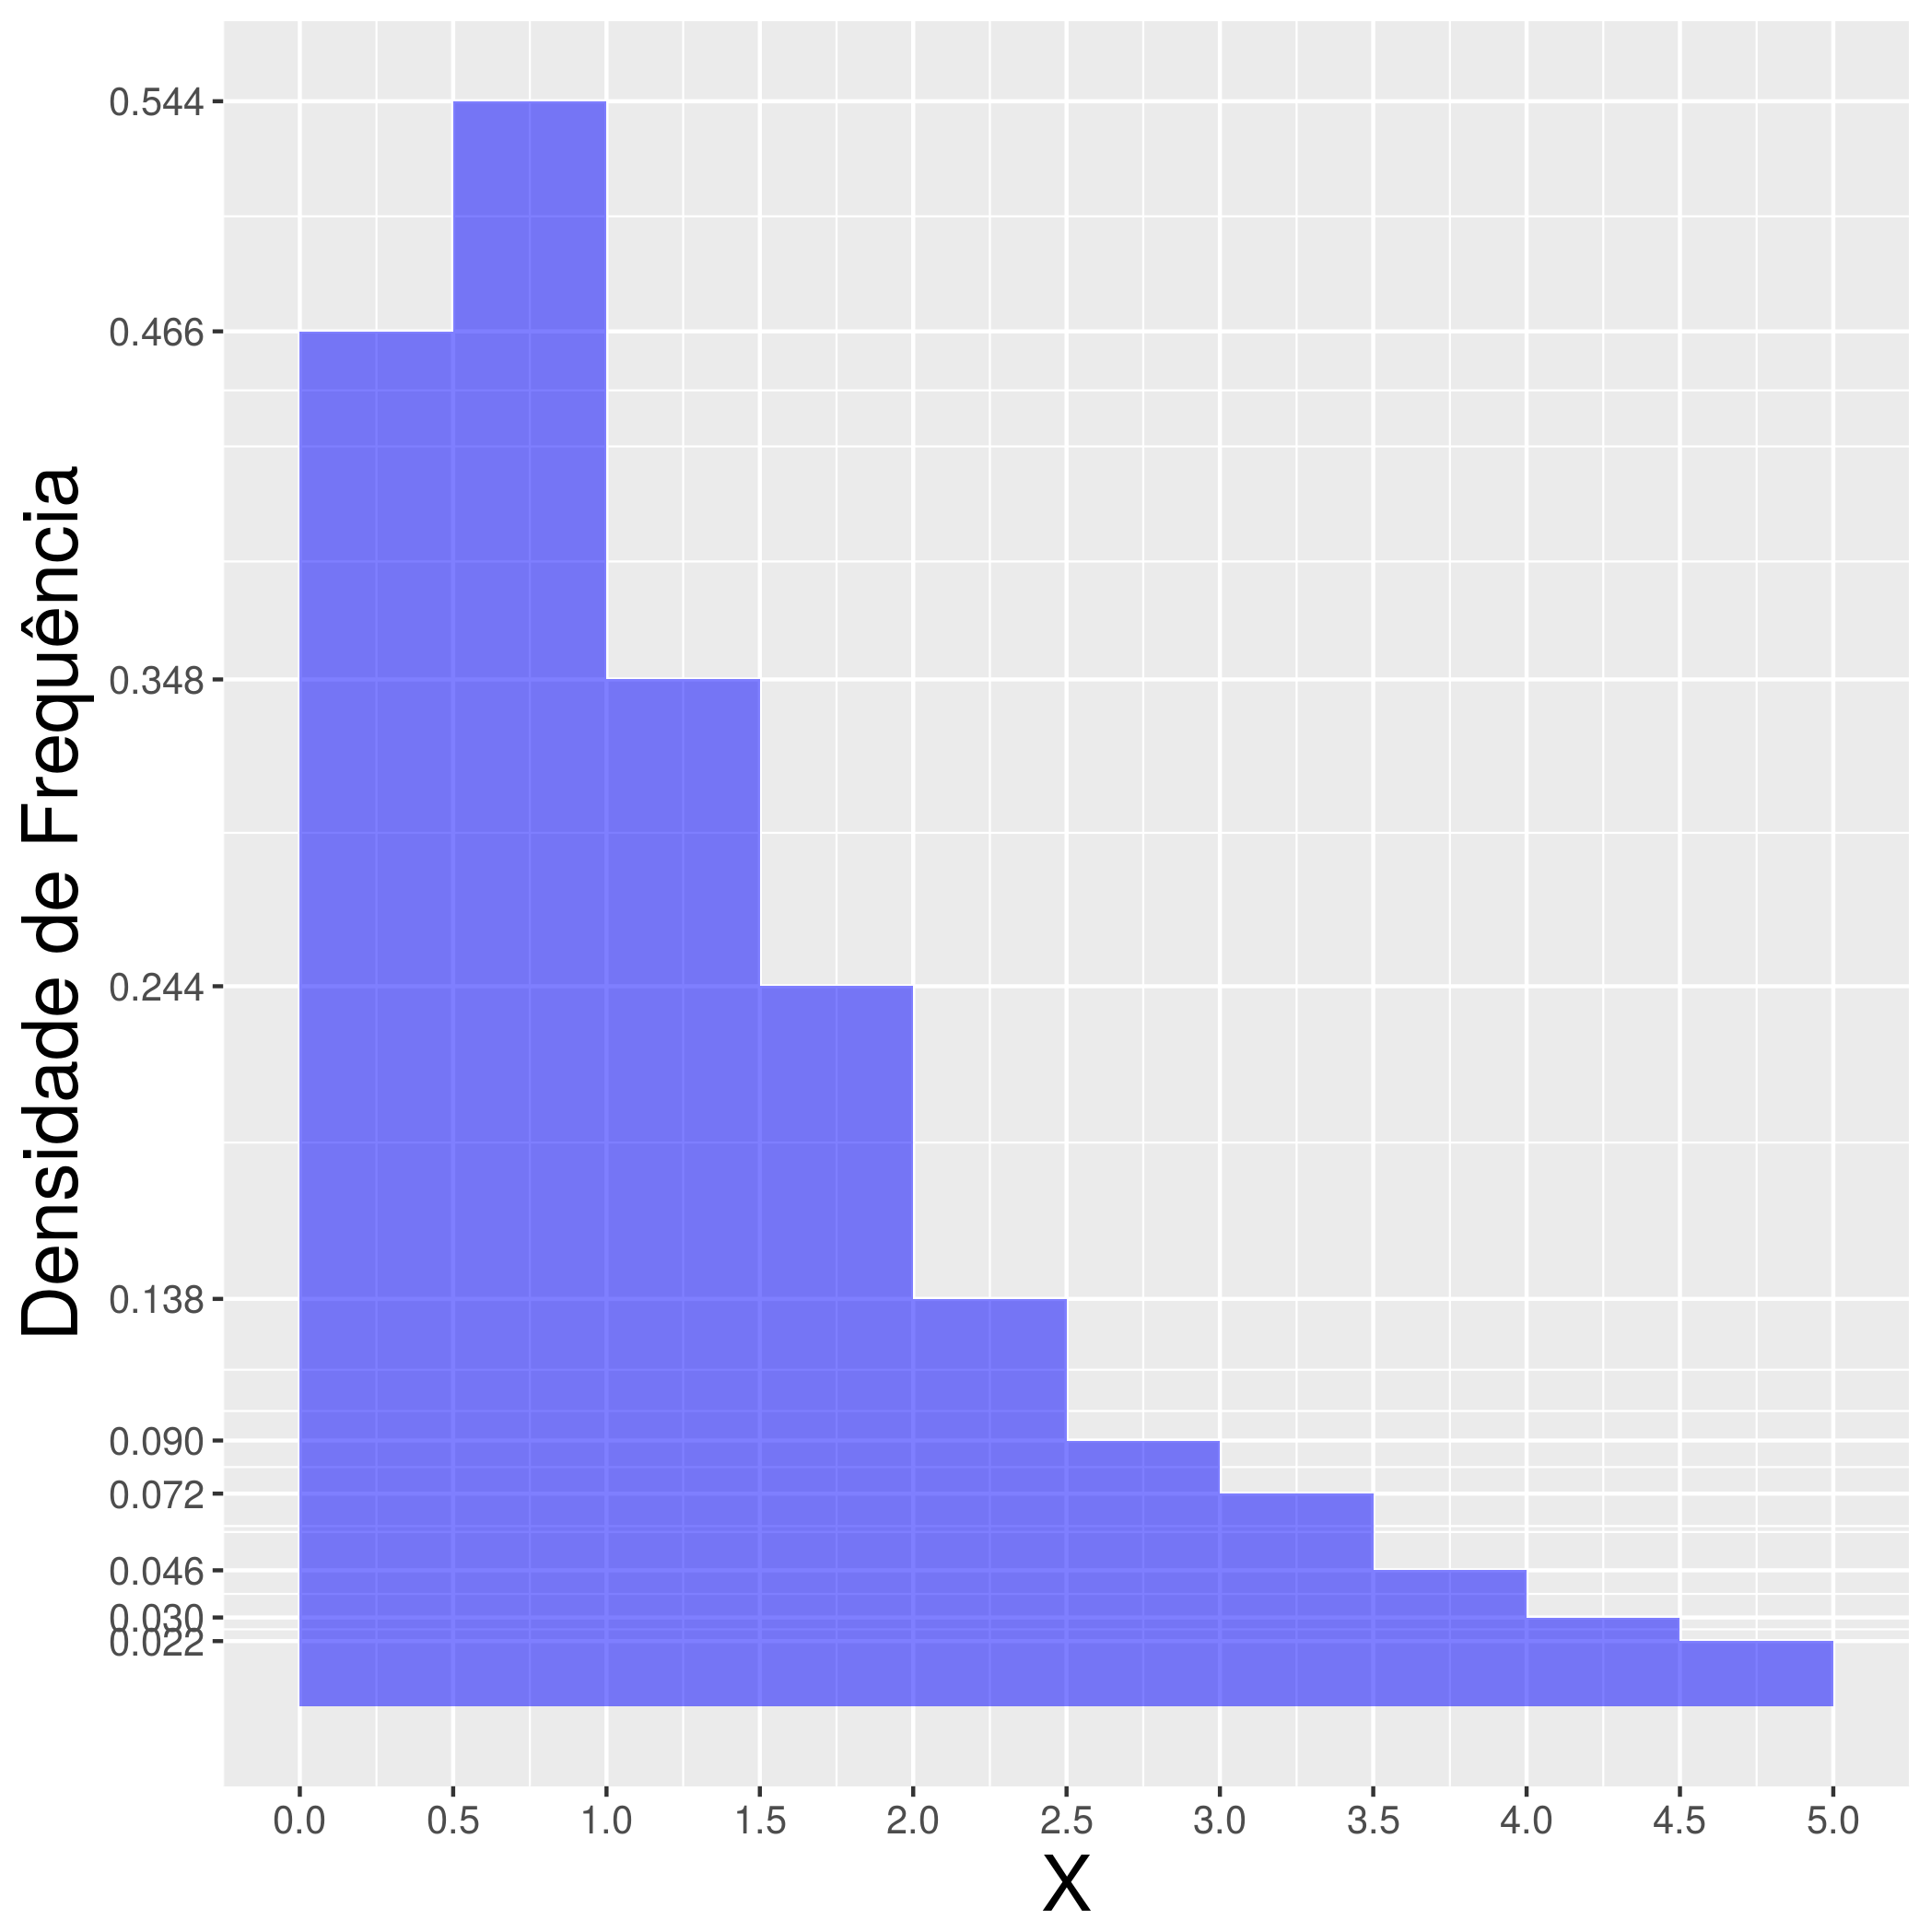
\includegraphics[width=10cm]{figure/X.png}
	\end{figure}    
	\begin{enumerate}
		\item Construa a tabela de distribuição de frequências.
		\item Construa o diagrama de caixa e o coeficiente de Bowley. Você julga que existe assimetria na variável quantitativa contínua $X$.
		\item Calcule o quantil de ordem $15\%$.
	\end{enumerate}
	
	\item Considere os alunos de duas turmas de Estatística Básica em um dado semestre da UFBA. O gráfico da Figura~\ref{fig:idade_estat} mostra o gráfico de barras da variável ``Idade''.
	\begin{figure}[htbp]
		\centering
		\caption{Idade para os alunos das duas turmas de Estatística Básica Básica.}
		\label{fig:idade_estat}
		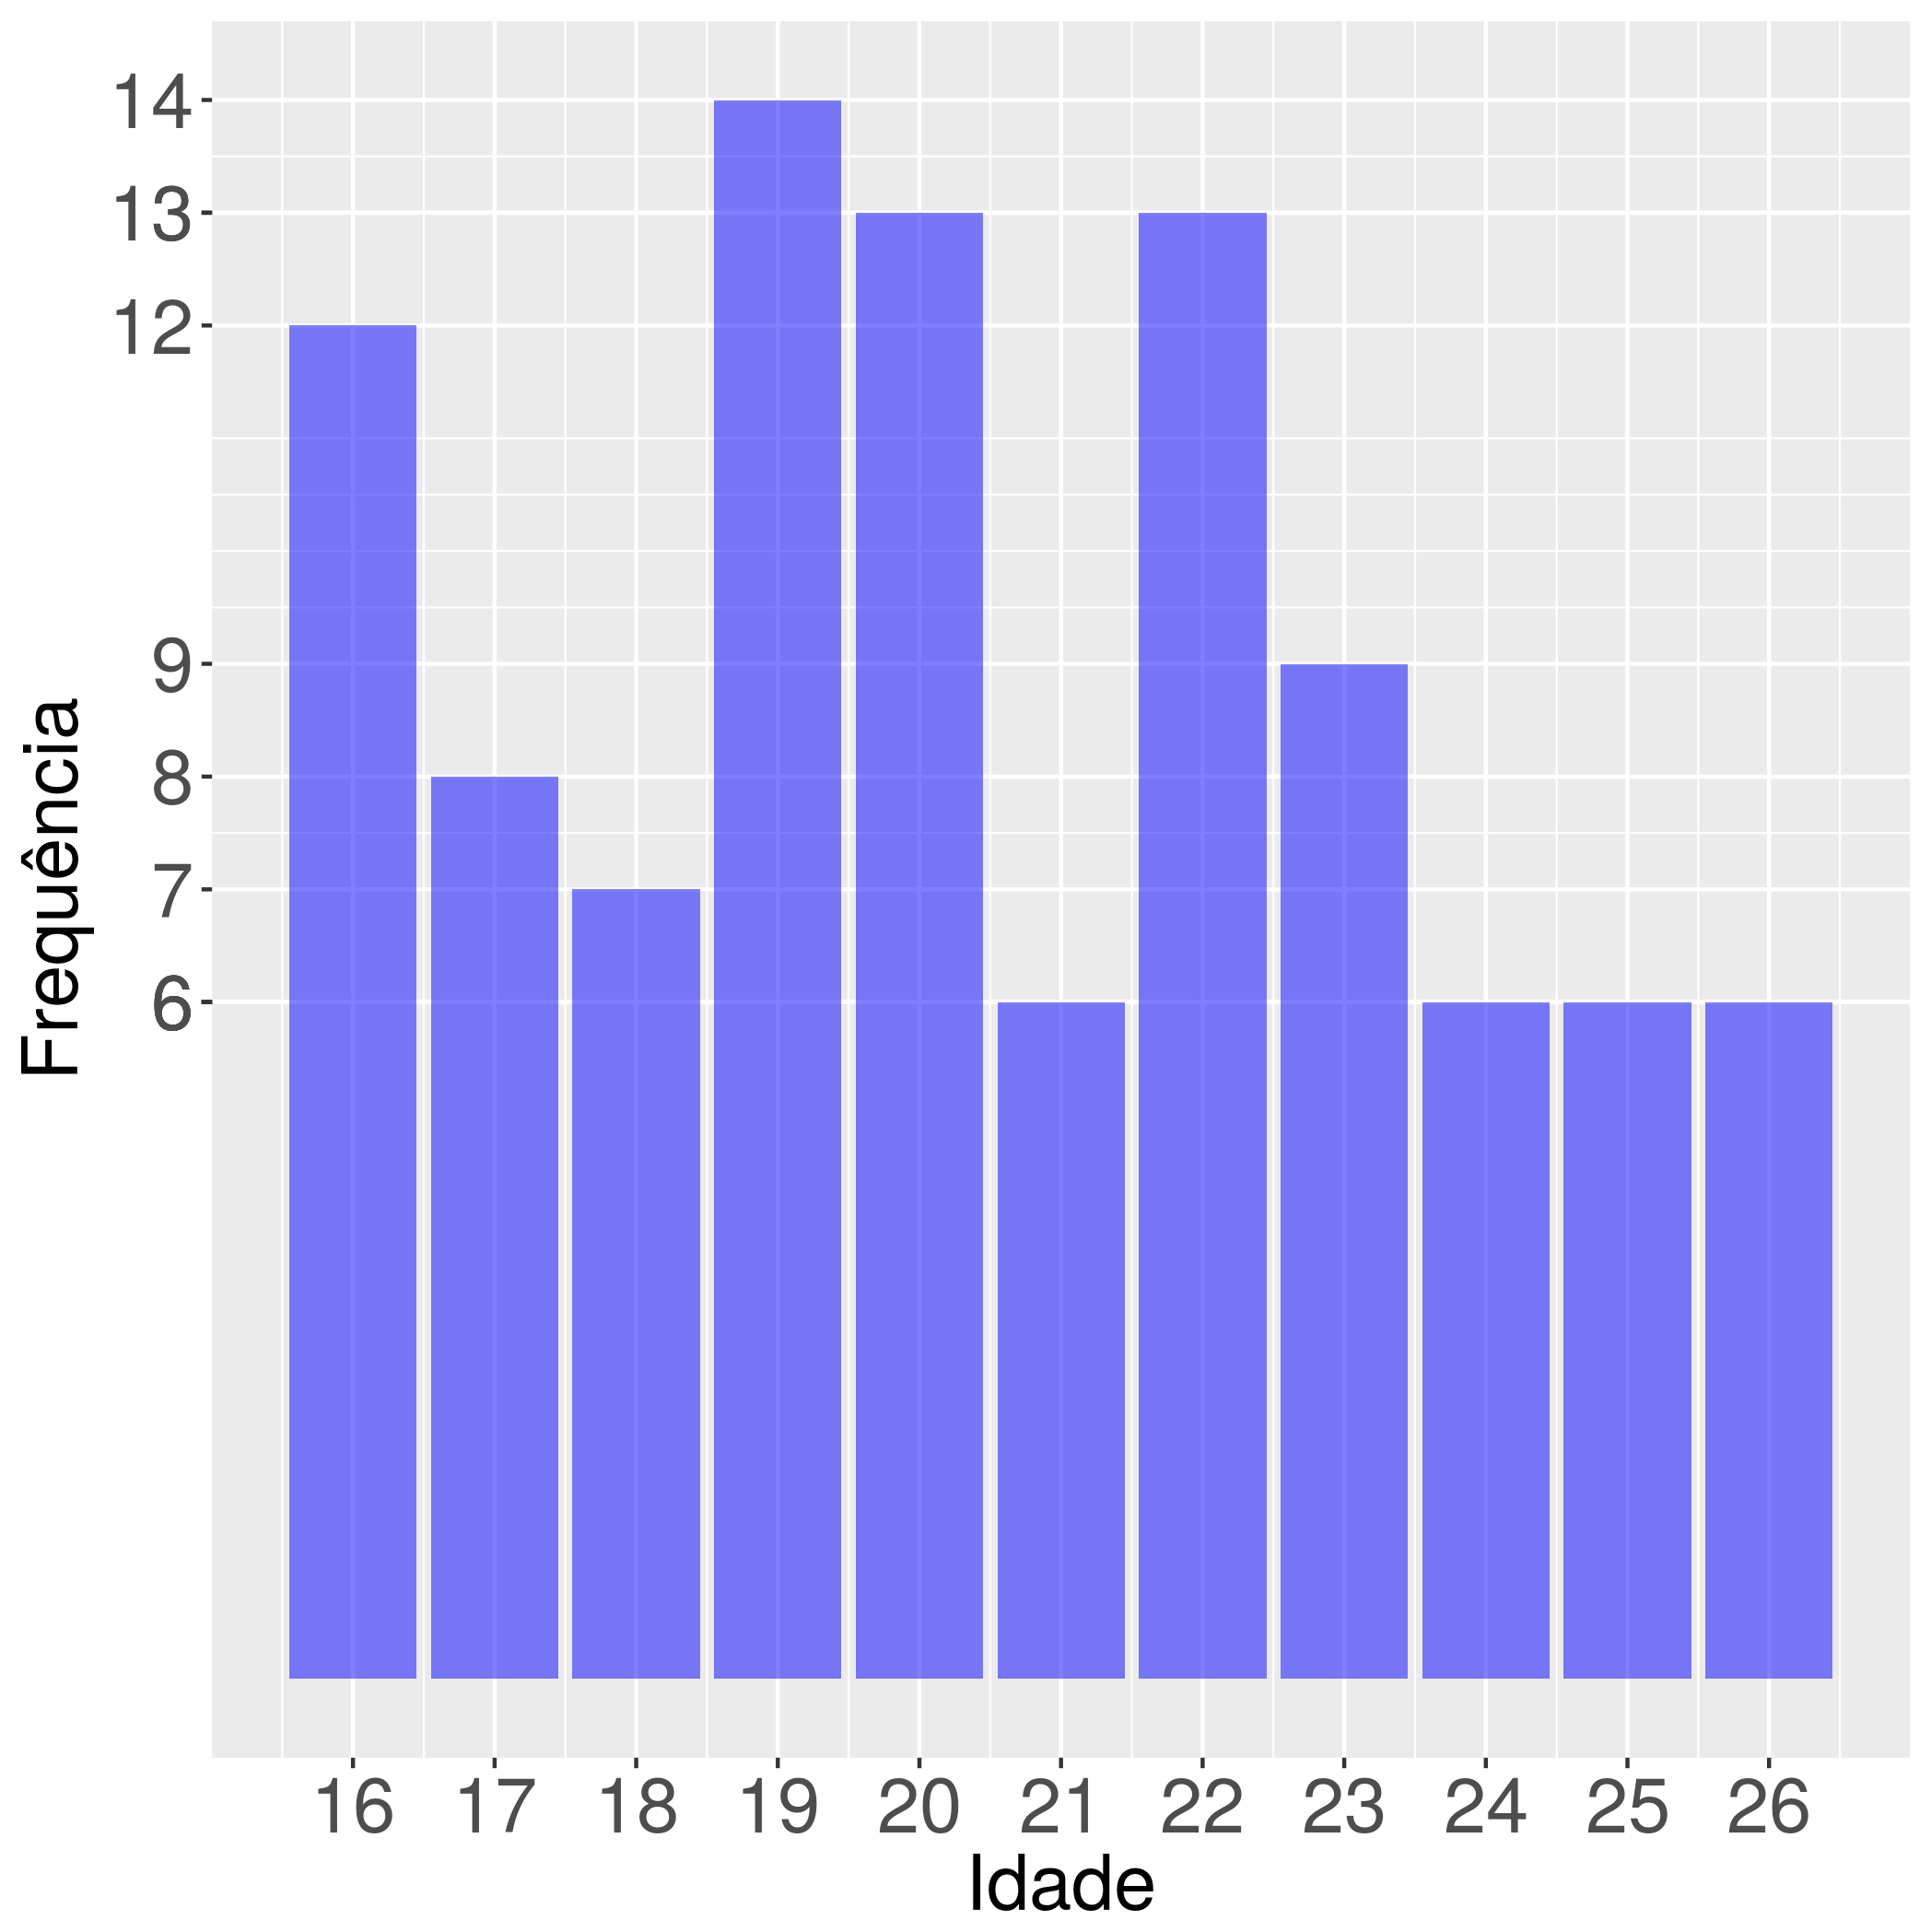
\includegraphics[width=10cm]{figure/Idade.png}
	\end{figure}
	\begin{enumerate}
		\item Construa a tabela de distribuição de frequências para a variáel quantitativa discreta ``Idade''.
		\item Construa o diagrama de caixa e o coeficiente de Bowley. Você julga que existe assimetria na variável quantitativa discreta ``Idade''.
		\item Qual a idade classifica um aluno entre os 20\% mais jovens.
		\item Qual a idade classifica um aluno entre os 15\% mais velhos.
	\end{enumerate}
	
	\item Alunos da Escola de Educação Física foram submetidos a um teste de resistência quanto ao número de quilômetros que conseguiram correr sem parar. Os dados estão apresentados na tabela~\ref{tab:resistencia}.
	\begin{table}[htbp]
		\centering
		\caption{Resistência dos alunos da Escola de Educação Física.}
		\label{tab:resistencia}
		\begin{tabular}{l|c}
			\toprule
			Faixas & Frequências \\ \midrule
			$0 |--- 4$ & 438\\
			$4 |--- 8$  & 206 \\
			$8 |--- 12$ & 125 \\
			$12 |--- 16$ & 22\\
			$16 |--- 20$ & 9 \\ \toprule
		\end{tabular}
	\end{table}
	\begin{enumerate}
		\item Qual é a variável em estudo?
		\item Construa o histograma.
		\item Determine o primeiro, o segundo e o terceiro quartil.
		\item Construa o diagrama de caixa e calcule o coeficiente de Bowley. Você diria que a variável do item (a) é simétrica?
	\end{enumerate}
	
	\item Vinte e uma pacientes de uma clínica médica tiveram o seu nível de potássio no plasma medido. Os resultados estão descritos na tabela~\ref{tab:potassio}.
	\begin{table}[htbp]
		\centering
		\caption{Nível de potássio no plasma.}
		\label{tab:potassio}
		\begin{tabular}{l|c}
			\toprule
			Nível & Frequência\\ \midrule
			$2,25 |---- 2,55$ & 1\\
			$2,55 |---- 2,75$ & 3\\
			$2,75 |---- 2,95$ & 2\\
			$2,95 |---- 3,15$ & 4\\
			$3,15 |---- 3,35$ & 5\\
			$3,35 |---- 3,65$ & 6\\ \toprule 
		\end{tabular}
		\begin{enumerate}
			\item Construa o histograma.
			\item Determine o primeiro, o segundo e o terceiro quartil.
			\item Construa o diagrama de caixa e calcule o coeficiente de Bowley. Você diria que existe assimetria nesta variável? Justifique a sua reposta.
			\item Qual a porcentagem de valores que estão acima do nível 3.
		\end{enumerate}
	\end{table}
	
	\item Foram feitas medições em operários da construção civil a respeito da taxa de hemoglobina no sangue (em gramas/cm$^3$) com resultados na tabela~\ref{tab:hemoglobina}.
	\begin{table}[htbp]
		\centering
		\caption{Taxa de hemoglobina nos operários.}
		\label{tab:hemoglobina}
		\begin{tabular}{cccccccccc}
			\toprule
			11,1 & 12,2 & 11,7 & 12,5 & 13,9 & 12,3 & 14,4 & 13,6 & 12,7 & 12,6 \\
			11,3 & 11,7 & 12,6 & 13,4 & 15,2 & 13,2 & 13,0 & 16,9 & 15,8 & 14,7 \\
			13,5 & 12,7 & 12,3 & 13,5 & 15,4 & 16,3 & 15,2 & 12,3 & 13,7 & 14,1 \\
			\bottomrule
		\end{tabular}
	\end{table}
	\begin{enumerate}
		\item Organize os dados em faixas de tamanho 1 a partir de 11.
		\item Construa o histograma.
		\item Determine o primeiro, o segundo e o terceiro quartil. (Use os dados brutos)
		\item Construa o diagrama de caixa e calcule o coeficiente de Bowley. Você diria que a taxa de hemoglobina nos operários tem assimetria? Justifique a sua resposta.
	\end{enumerate}
	
	\item A tabela~\ref{tab:criancas} apresenta as frequências relativas de ocorrências de faixas de altura (em cm) para uma amostra de 100 crianças de 12 anos de idade.
	\begin{table}[htbp]
		\centering
		\caption{Altura de 100 crianças com 12 anos.}
		\label{tab:criancas}
		\begin{tabular}{l|c}
			\toprule
			Faixas & Frequência relativa \\ \midrule
			$100 |---- 110$ & 0,10 \\ 
			$110 |---- 120$ & 0,25 \\
			$120 |---- 130$ & 0,30 \\
			$130 |---- 140$ & 0,25 \\
			$140 |---- 160$ & 0,10 \\ \toprule
		\end{tabular}
	\end{table}
	
	\begin{enumerate}
		\item Construa o histograma.
		\item Construa o diagrama de caixa e calcule o coeficiente de Bowley. Você julga que a altura das crinças tem assimetria? Justifique a sua resposta.
		\item Desejando-se separar os $15\%$ mais altos, qual seria o ponto de corte?
	\end{enumerate}
		
\end{enumerate}

\end{document}
